\documentclass{article}
\usepackage[a4paper]{geometry}
\usepackage{fancyhdr} 
\usepackage{tikz}
\usepackage{hyperref} 
\pagestyle{fancy}
\lhead{Lagebeziehungen zwischen zwei Ebenen}
\rhead{Juli 2025}
\begin{document}
 
\newcommand{\vect}[1]{\overrightarrow{#1}}
  
\section{Lagebeziehungen zwischen zwei Ebenen}
Die Langebeziehung zwischen zwei Ebenen, $\mathrm{E}_1$ und $\mathrm{E}_2$, beschreibt wie diese zueinander im Raum stehen. Dabei gibt es drei Möglichkeiten.
\begin{description}
 \item[Schneidung] Wenn zwei Ebenen sich schneiden, kommt es zu einer Schnittgerade; der Gerade, auf welcher alle Punkte liegen, welche auf beiden Gerade gleichzeitig liegen. Dies passiert zwangsweise, wenn die Normalvektoren der beiden Geraden, $\vect{n_1}$ und $\vect{n_2}$, nicht kollinear zueinander sind.
 \item[identisch] Sind alle Punkte der Ebene $\mathrm{E}_1$ auch Teil der Ebene $\mathrm{E}_2$, so sind die beiden Ebenen identisch. Dies bedeutet, dass ihre beiden Normalvektoren zwangsweise kollinear zueinander sein müssen.
 \item[echt parallel] Zwei Ebenen sind zueinander echt parallel, wenn sie keinen gemeinsamen Punkt teilen. Auch hier müssen zwangsweise die Normalvektoren der Ebenen kollinear sein.
\end{description}
 
\begin{center}
 \begin{tabular}{c c c}
  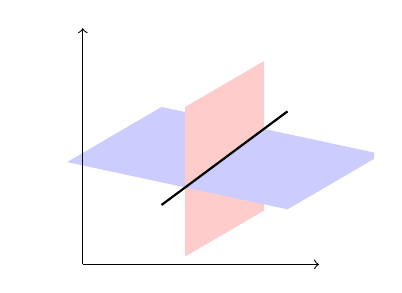
\begin{tikzpicture}
   \begin{scope}  
    \clip(-0.7,0) rectangle (3.7,3);
    \fill[blue!20] (-0.2, 1.3) -- (1.0, 2.0) -- (3.8, 1.4) -- (2.6, 0.7) -- cycle;
    \fill[red!20] (1.3, 0.1) -- (1.3, 2) -- (2.3, 2.583) -- (2.3, 0.683) -- cycle; 
    \fill[blue!20] (1.3, 0.978) -- (2.3, 1.721) -- (2.3, 0.764) -- cycle; 
   \end{scope}
   
   \draw[thick,black] (1.3-0.3,0.978 - 0.3*0.743) -- ++(1.6, 1.6*0.743); 
   \draw[->] (0, 0) -- (3, 0); 
   \draw[->] (0, 0) -- (0, 3);
  \end{tikzpicture}
  &
  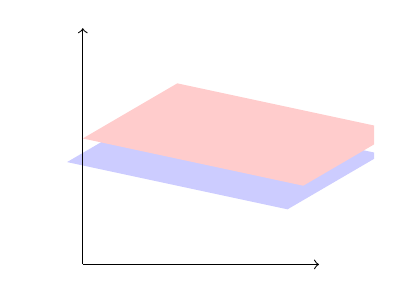
\begin{tikzpicture}
   \begin{scope}  
    \clip(-0.7,0) rectangle (3.7,3);
    \fill[blue!20] (1.2-0*1.2-1.4,1-0*0.7+0.3) -- (1.2+1*1.2-1.4,1+1*0.7+0.3) -- (1.2+1*1.2+1.4,1+1*0.7-0.3) -- (1.2-0*1.2+1.4,1-0*0.7-0.3) -- cycle;
    \fill[red!20] (1.4-0*1.2-1.4,1.3-0*0.7+0.3) -- (1.4+1*1.2-1.4,1.3+1*0.7+0.3) -- (1.4+1*1.2+1.4,1.3+1*0.7-0.3) -- (1.4-0*1.2+1.4,1.3-0*0.7-0.3) -- cycle;
   \end{scope}
  
   \draw[->] (0, 0) -- (3, 0); 
   \draw[->] (0, 0) -- (0, 3);
  \end{tikzpicture} 
  &
  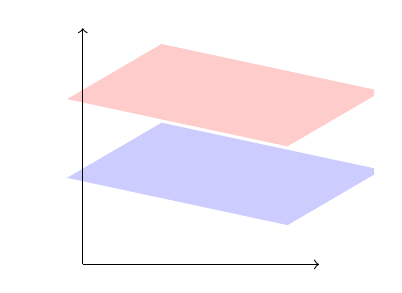
\begin{tikzpicture}
   \begin{scope}  
    \clip(-0.7,0) rectangle (3.7,3);
    \fill[blue!20] (1.2-0*1.2-1.4,0.8-0*0.7+0.3) -- (1.2+1*1.2-1.4,0.8+1*0.7+0.3) -- (1.2+1*1.2+1.4,0.8+1*0.7-0.3) -- (1.2-0*1.2+1.4,0.8-0*0.7-0.3) -- cycle;
    \fill[red!20] (1.2-0*1.2-1.4,1.8-0*0.7+0.3) -- (1.2+1*1.2-1.4,1.8+1*0.7+0.3) -- (1.2+1*1.2+1.4,1.8+1*0.7-0.3) -- (1.2-0*1.2+1.4,1.8-0*0.7-0.3) -- cycle;
   \end{scope} 
     
   \draw[->] (0, 0) -- (3, 0); 
   \draw[->] (0, 0) -- (0, 3);
  \end{tikzpicture} 
  \\
  Schneidung & identisch & echt parallel \\
  $\vect{n_1}$ und $\vect{n_2}$ nicht kollinear &
  $\vect{n_1}$ und $\vect{n_2}$ kollinear, &
  $\vect{n_1}$ und $\vect{n_2}$ kollinear, \\
  eine Schnittgerade & alle Punkte von $\mathrm{E}_1$ in $\mathrm{E}_2$ & kein gemeinsamer Punkt
 \end{tabular} 
\end{center}
\subsection{Bestimmen}
Weil alle drei Lagebeziehungen unterschiedliche gleiche Punkte haben, kann die Lagebeziehung zwischen zwei Ebenen basierend auf einzig und allein ihrer gleichen Punkte bestimmt werden.
 
Stellt sich beim Gleichsetzen der Ebenengleichungen heraus, dass es keinen gemeinsamen Punkt gibt, unter anderem dadurch, dass es beim auflösen zu einem Widerspruch kommt, so ist sind die Ebenen echt parallel zueinander. Sind die Gleichungen aber gleich, kommt es zu einer Identität, sind die beiden Ebenen auch identisch. Kommt es beim Auflösen der Gleichung oder des \hyperref[Lineare Gleichungssysteme]{Linearen Gleichungssystems} dazu, dass die Koordinaten aller gleichen Punkte in Abhängigkeit von nur einem Parameter gesetzt werden können, so liegen all diese auf der Schnittgerade. Desweiteren kann die Schnittgerade gefunden werden, indem alle Koordinaten in Abhängigkeit von nur einem Parameter aufgestellt werden. 
 
\end{document} 
 
 
 
